\documentclass[a4paper]{jsarticle}
\usepackage[dvipdfmx]{graphicx}
\usepackage{amsmath}
\usepackage{bm}
\renewcommand{\thesection}{第\arabic{section}問}
\renewcommand{\thesubsection}{(\arabic{subsection})}
\renewcommand{\thesubsubsection}{(\alph{subsubsection})}
\begin{document}

\title{2014分野1}
\author{nakao}
\maketitle

\section{}
わーーー
\section{}
糸の張力を$T$とすると、鉛直方向と垂直方向の運動方程式はそれぞれ、
\begin{align}
  m \frac{\mathrm{d}^2}{\mathrm{d} t^2} (l \cos \theta)
  &= mg - T \cos \theta \\
  m \frac{\mathrm{d}^2}{\mathrm{d} t^2} (l \sin \theta)
  &= - T \sin \theta
\end{align}
で与えられる。ここに$\cos \theta \simeq 1, \sin \theta \simeq \theta$を代入すると、
\begin{align}
  mg - T &= 0 \\
  m l \ddot{\theta} &= -T \theta 
\end{align}
となる。これらより$T$を消去して、
\begin{equation}
  m l \ddot{\theta} = -m g \theta
\end{equation}
を得る。$x = l \sin \theta \simeq l \theta$より、
$\theta = x / l, \ddot{\theta} = \ddot{x} / l$が成り立ち、これらを式(4)に代入して、
\begin{equation}
  \ddot{x} = -\frac{g}{l} x
\end{equation}
が得られる。したがって、この運動の角振動数$\omega_0$は、
$\omega_0 = \sqrt{g/l}$である。

\subsection{}
運動方程式は、
\begin{equation}
  \begin{aligned}
    m \ddot{x}_1 &= -\frac{mg}{l} x_1 - k(x_1 - x_2) \\
    m \ddot{x}_2 &= -\frac{mg}{l} x_2 - k(x_2 - x_1)
  \end{aligned}
\end{equation}
であり、行列表示すると、
\begin{equation}
  \begin{pmatrix}
    m & 0 \\
    0 & m \\
  \end{pmatrix}
  \begin{pmatrix}
    \ddot{x}_1 \\ \ddot{x}_2
  \end{pmatrix} +
  \begin{pmatrix}
    \frac{mg}{l} + k & -k \\
    -k & \frac{mg}{l} + k
  \end{pmatrix} = \boldsymbol{0}
\end{equation}
と表せる。\par
行列$M,K$を
\begin{equation}
  M =
  \begin{pmatrix}
    m & 0 \\
    0 & m \\
  \end{pmatrix},\quad
  K =
  \begin{pmatrix}
    \frac{mg}{l} + k & -k \\
    -k & \frac{mg}{l} + k
  \end{pmatrix}
\end{equation}
で定義し、固有振動数$\omega$と固有モード$\boldsymbol{\phi}$に対して、
\begin{equation}
  (K - \omega^2 M) \boldsymbol{\phi} = \boldsymbol{0}
\end{equation}
が成り立つ。$\boldsymbol{\phi} \neq \boldsymbol{0}$なる解が存在するためには、
\begin{equation}
  \det (K - \omega^2 M) = 0
\end{equation}
が必要である。ここで、
\begin{equation}
  \det (K - \omega^2 M) = \det
  \begin{pmatrix}
    \frac{mg}{l} + k - \omega^2 m & -k \\
    -k & \frac{mg}{l} + k - \omega^2 m
  \end{pmatrix} =
  \left(\frac{mg}{l} + 2k - \omega^2 m\right)
  \left(\frac{mg}{l} - \omega^2 m\right)
\end{equation}
より、
\begin{equation}
  \omega = \sqrt{\frac{g}{l}}, \sqrt{\frac{g}{l} + \frac{2k}{m}}
\end{equation}
であればよい。\par
$\omega = \sqrt{g/l}$のとき、
$(K - \omega^2 M) \boldsymbol{\phi} = \boldsymbol{0}$
を解くと、$\boldsymbol{\phi} \propto (1, 1)$であるから、これを1次モードとすると、
\begin{equation}
  \omega_1 = \sqrt{\frac{g}{l}},\quad
  \boldsymbol{\phi}_1 =
  \begin{pmatrix}
    1 \\ 1
  \end{pmatrix}
\end{equation}
である。このとき固有周期$T_1$は、
\begin{equation}
  T_1 = 2 \pi \sqrt{\frac{l}{g}}
\end{equation}
である。\par
$\omega = \sqrt{g/l + 2k/m}$のとき、
$(K - \omega^2 M) \boldsymbol{\phi} = \boldsymbol{0}$
を解くと、$\boldsymbol{\phi} \propto (1, -1)$であるから、これを2次モードとすると、
\begin{equation}
  \omega_2 = \sqrt{\frac{g}{l} + \frac{2k}{m}},\quad
  \boldsymbol{\phi}_2 =
  \begin{pmatrix}
    1 \\ -1
  \end{pmatrix}
\end{equation}
である。このとき固有周期$T_2$は、
\begin{equation}
  T_2 = 2 \pi \sqrt{\frac{ml}{mg + 2kl}}
\end{equation}
である。\par
モード形の概形は図1,2の通り。
1次モードでは2つのおもりが同一方向、2次モードでは2つのおもりが反対方向に運動する。
\begin{figure}[htb]
  \begin{minipage}{0.5\hsize}
    \centering
    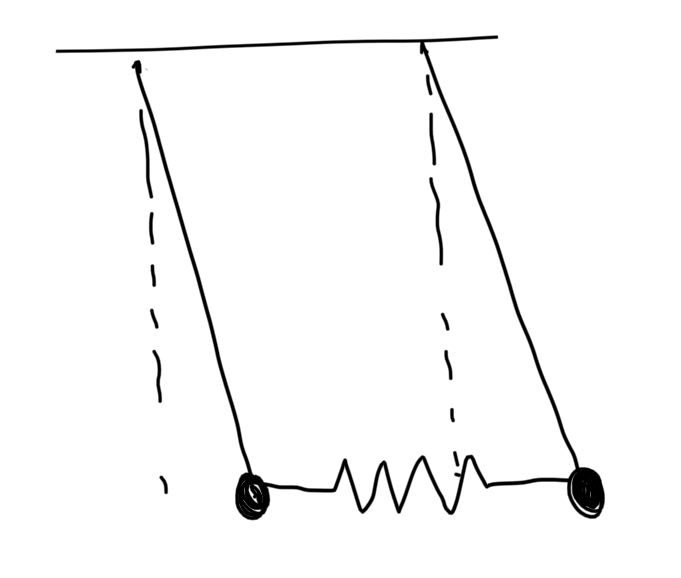
\includegraphics[width=0.5\hsize]{fig1.png}
    \caption{1次モードの概形}
  \end{minipage}
  \begin{minipage}{0.5\hsize}
    \centering
    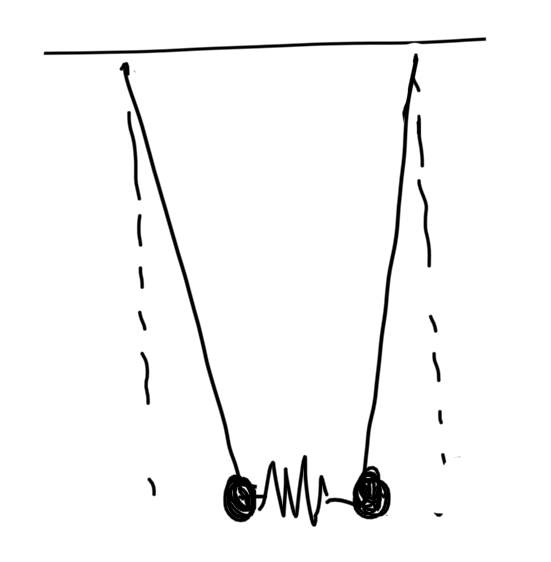
\includegraphics[width=0.5\hsize]{fig2.png}
    \caption{2次モードの概形}
  \end{minipage}
\end{figure}
\subsection{}
おもりの変位を固有振動の重ね合わせとして、
\begin{equation}
  \boldsymbol{x} =
  \begin{pmatrix}
    x_1 \\ x_2
  \end{pmatrix} =
  q_1 \boldsymbol{\phi}_1 + q_2 \boldsymbol{\phi}_2
\end{equation}
と表す。$q_1, q_2$は時間変化するスカラーである。
これを運動方程式$M \ddot{\boldsymbol{x}} + K \boldsymbol{x} = \boldsymbol{0}$に代入し、固有モードの直交性を用いると、
\begin{equation}
  \begin{aligned}
    2 m \ddot{q}_1 + \frac{2mg}{l} q_1 = 0 \\
    2 m \ddot{q}_2 + \left(\frac{2mg}{l} + 4k\right) q_2 = 0
  \end{aligned}
\end{equation}
が得られる。初期条件は
$\boldsymbol{x}(0) = (\alpha, 3 \alpha), \dot{\boldsymbol{x}}(0) = (0, 0)$
より、
\begin{equation}
  \begin{aligned}
    q_1(0) = 2 \alpha, \quad \dot{q}_1(0) = 0 \\
    q_2(0) = -\alpha, \quad \dot{q}_2(0) = 0
  \end{aligned}
\end{equation}
式(19),(20)を解くと、
\begin{equation}
  \begin{aligned}
    q_1 &= 2 \alpha \cos \sqrt{\frac{g}{l}} t \\
    q_2 &= -\alpha \cos \sqrt{\frac{g}{l} + \frac{2k}{m}} t
  \end{aligned}
\end{equation}
が得られる。よって、
\begin{equation}
  \begin{aligned}
    \boldsymbol{x} &= 2 \alpha \cos \sqrt{\frac{g}{l}} t
    \begin{pmatrix}
      1 \\ 1
    \end{pmatrix} -\alpha \cos \sqrt{\frac{g}{l} + \frac{2k}{m}} t
    \begin{pmatrix}
      1 \\ -1
    \end{pmatrix} \\
    &=
    \begin{pmatrix}
      2 \alpha \cos \sqrt{\frac{g}{l}} t -\alpha \cos \sqrt{\frac{g}{l} + \frac{2k}{m}} t \\
      2 \alpha \cos \sqrt{\frac{g}{l}} t +\alpha \cos \sqrt{\frac{g}{l} + \frac{2k}{m}} t
    \end{pmatrix}
  \end{aligned}
\end{equation}
である。
\subsection{}
モード解析により系の固有振動数が得られ、環境から系に与えられる振動が固有振動数に近いかという単純な指標で大まかな安全性を見ることができる。
瞬間的に動的変位は静的変位よりかなり大きくなるため、特に共鳴が起きないかを見ることは重要である。
\end{document}